\documentclass[a4paper,12pt]{article}
\usepackage[utf8]{inputenc}

\usepackage[utf8]{inputenc}
\usepackage[T2A]{fontenc}
\usepackage[russian]{babel}
\usepackage{amsthm}
\usepackage{amsmath}
\usepackage{amssymb}
\usepackage{tikz}
\usepackage{textcomp}
\usepackage{marvosym}
\usepackage{ esint }
\setlength{\topmargin}{-0.5in}
\setlength{\textheight}{9.1in}
\setlength{\oddsidemargin}{-0.4in}
\setlength{\evensidemargin}{-0.4in}
\setlength{\textwidth}{7in}
\setlength{\parindent}{0ex}
\setlength{\parskip}{1ex}
\newcommand{\ndiv}{\hspace{-4pt}\not|\hspace{2pt}}
\usepackage{graphicx}
\usepackage{float}
\usepackage{wrapfig}
\usepackage{derivative}
\usepackage{multirow}
\usepackage{physics}
\graphicspath{ {./images/} }
%%% Заголовок

\title{Лабораторная работа № 4.1.1\\Изучение центрированных оптических систем}
\author{Пазов Тенгиз, Симухин Егор}
\date{Март 2025}

\begin{document}
\maketitle
\newpage

\textbf{Цель:} изучить методы определения фокусных расстояний
линз и сложных оптических систем; определить характеристики оптической системы, составленной из тонких линз; изучить недостатки
реальных линз — сферическую и хроматическую аберрации.

\textbf{Оборудование:} : оптическая скамья с набором рейтеров, положительные и отрицательные линзы, экран, осветитель с ирисовой
диафрагмой, зрительная труба, светофильтры, кольцевые диафрагмы, линейка.

\section{Теоретические сведения}
\subsection*{Определения фокусных расстояний}
Формула тонкой линзы имеет вид
\begin{equation}
    \frac{1}{f} = \frac{1}{a} + \frac{1}{b},
\end{equation}
\noindent
где $f$ -- фокусное расстояние, $a$ -- расстояния от предмета до линзы, $b$ -- расстояние от изображения до линзы.

\noindent
Для измерения фокусного расстояния тонкой собирающей линзы может использоваться схема см. рис. 1. и формула (2).
\begin{equation}
    f = \frac{L^2 - l^2}{4L}
\end{equation}

\begin{figure}[H]
    \centering
    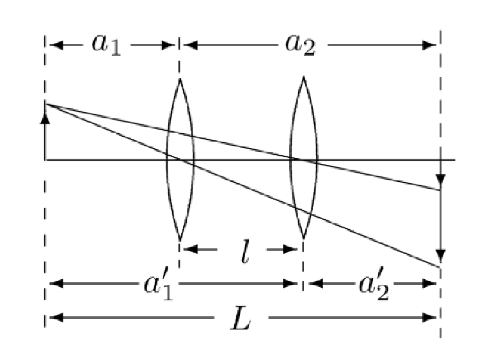
\includegraphics[scale=0.7]{1.png}
    \caption{Схема измерения фокуса тонкой собирающей линзы}
\end{figure}

\noindent
Также фокусное расстояние тонкой собирабщей линзы можно измерить с помощью зрительной трубы, настроенной на бесконечность. Если расположить линзу между предметом и трубой и найти четкое изображение предмета, то расстояние от линзы до предмета будет равно фокусному.

\noindent
Для определения расстояния тонкой рассеивающей линзы воспользуемся схемой на рис. 2 и формулой тонкой линзы. Также можно воспользоваться зрительной трубой, настроенной на бесконечность. Если расположить предмет у нее в фокусе, то изображение переместиться в бесконечность, что можно проверить с помощью зрительной трубы.

\begin{figure}[H]
    \centering
    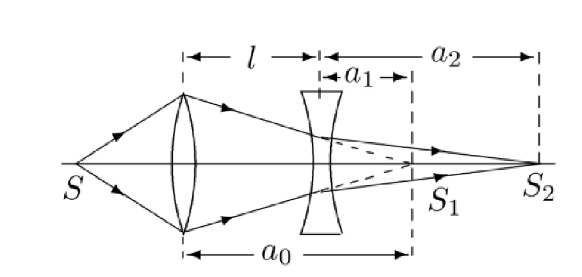
\includegraphics[scale=0.7]{2.png}
    \caption{Схема измерения фокуса тонкой рассеивающей линзы}
\end{figure}

\noindent
Для определения фокусного расстояния и положения главных плоскостей сложной оптической системы может использоваться метод Аббе: схема на рис. 3 и формула (3).

\begin{figure}[H]
    \centering
    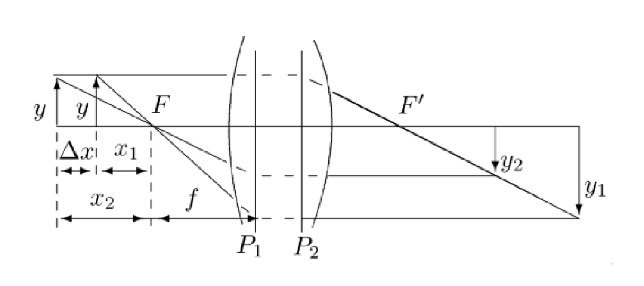
\includegraphics[scale=0.7]{3.png}
    \caption{Схема определения фокусного расстояние и положения главных плоскостей сложной оптической}
\end{figure}

\begin{equation}
    f = \frac{\Delta x}{y / y_1 - y / y_2}    
\end{equation}

\newpage
\section{Ход Работы}
\subsection*{Центрировка элементов оптической системы}
\textbf{1.} Выделим из всех линз собирающие и рассеивающие. 

\textbf{2.} Получая изображение удалённого объекта(в нашем случае света ламп), оценим фокусное расстояние всех линз(таким образом также можно определить рассеивающую линзу, т.к. она не будет давать действительного изображения). Для отрицательной линзы можно оценить фокусное расстояние, совместив её с положительной линзой. 

\textbf{3.} Полученные оценки занесём в таблицу

\begin{table}[H]
\centering
	\begin{tabular}{|c|c|c|}
	\hline
	№ линзы & тип линзы & F, см \\ \hline
	4.1 & собирающая & 5 \\ \hline
	4.2 & собирающая & 10 \\ \hline
	4.4 & собирающая & 15 \\ \hline
	4.5 & рассеивающая &  \\ \hline
	4.6 & собирающая & 5 \\ \hline
	\end{tabular}
\end{table}

\textbf{4.} Соберём и отцентрируем установку.

\subsection*{Определение фокусных расстояний линз с помощью подзорной трубы}
\textbf{1.} Настроим подзорную трубу так, чтобы она была настроена на "бесконечность".

\textbf{2.} Установим подзорную трубу на установку, между предметом и трубой поставим собирающую линзу так, чтобы её расстояние до предмета было примерно равно оценённому ранее фокусному.

\textbf{3.} Слегка перемещая линзу, добьёмся чёткого изображения, нанесённого на транспарант источника, измерим расстояние от источника до линзы - фокусное расстояние - и, проделав то же самое для остальных линз, занесём в таблицу. Также развернём линзы в другую сторону и проверим, совпадает ли фокусное расстояние с ранее полученным(можно ли считать линзы тонкими).
F - линза обращена прямой стороной к источнику.
$F_{rot}$ - линза обращена прямой стороной к под-ой трубе.
\begin{table}[H]
\centering
	\begin{tabular}{|c|c|c|c|} 
	\hline
	№ линзы & тип линзы & F, см & $F_{rot}$, см \\ \hline
	4.1 & собирающая & 7,6 & 7,2 \\ \hline
	4.2 & собирающая & 12,5 & 12,5 \\ \hline
	4.3 & собирающая & 17,4 & 17,4 \\ \hline
	4.4 & собирающая & 25 & 24,3 \\ \hline
	4.6 & собирающая & 4.25 & 5.95 \\ \hline
	\end{tabular}
\end{table}
В таблице в линзе 4.2 записаны средние значения для n измерений, произведенных с данной линзой.
При повороте у линз практически не меняется фокусное расстояние, что говорит о возможности их считать тонкими.

\textbf{4.} Для линзы 4.2 измерим обратное($F_{rot}$) и прямое($F$) фокусное расстояние ещё несколько раз, чтобы оценить среднеквадратичные отклонения, соответственно равные $\sigma_{F} = 0,32$ см, $\sigma_{F_{rot}} = 0,23$

\textbf{5.} Теперь измерим фокусное расстояние отрицательной линзы. Для этого разместим на скамье вспомогательную линзу(в нашем случае линзу 1.1) так, чтобы получить на экране чёткое изображение. Измерим расстояние от этой линзы до экрана. $a_0 = 22,0 \pm 0,2$ см.

\textbf{6.} Между экраном и собирающей линзой установим отрицательную, далее уберём экран, установим на скамье зрительную трубу. Меняя положение рассеивающей линзы, добьёмся сфокусированного изображения в поздорной трубе. Измерим расстояние между положительной и отрицательной линзами. $l = 12,7 \pm 0,3$ см.

\textbf{7.} Получим значение фокусного расстояние рассеивающей линзы 1.5 $F_{1.5} = l - a_0 = -9,3 \pm 0,4$ см.

\subsection*{Измерение фокусных расстояний линз по формуле тонкой линзы и методом Бесселя}
\textbf{1.} Установим одну из линз(в нашем случае была выбрана линза 4.2) между экраном и источником. Экран же расположим на расстоянии $L \sim 1,2 \cdot 4F_{4.6}$. $L = 60 \pm 0,1$ см.

\textbf{2.} Перемещая линзу, получим 2 различных действительных изображения - увеличенное и уменьшенное. Измерим для каждого из случаев расстояние от линзы до источника $s_1 = 16,4 \pm 0,1$ см и $s_2 = 42 \pm 0,1$ см. $l = s_2 - s_1 = 25,6 \pm 0,14$ см.

\textbf{3.} Теперь по формуле тонкой линзы и по формуле Бесселя найдём фокусное расстояние линзы(формулы (1) и (2)). Получилось 3 значения фокусного расстояния.
$F_1 = 11.92 \pm 0,05$ см, $F_2 = 12.6 \pm 0,06$ см, $F_\text{Б} = 12.27 \pm 0,04$ см.

\textbf{4.} Теперь для повернутой на 180 градусов линзы.
$F_1 = 12.00 \pm 0,05$ см, $F_2 = 12.63 \pm 0,06$ см, $F_\text{Б} = 12.332 \pm 0,04$ см.
\subsection*{Измерение фокусных расстояний методом Аббе}
\textbf{1.} Установим линзу(в нашем случае линза 4.2) между осветителем с транспарантом и экраном. На источнике есть предмет, линейный размер измерим линейкой $y_0 = 2.2 \pm 0,1$ см. 

\textbf{2.} Перемещая линзу вдоль скамьи, найдём положение действительного изображения на экране и измерим его линейный размер
\textbf{3.} Оставляя линзу в прежнем положении, сдвинем источник на $\Delta x$. 

\textbf{4.} Теперь сместим нашу линзу так, чтобы вновь получить действительное изображение. Данное смещение равно $\Delta x'$. Измерим новый линейный размер изображения $y_2$.

\textbf{5.} Вычислим значение фокусного расстояния методом Аббе.
\begin{figure}[H]
    \centering
    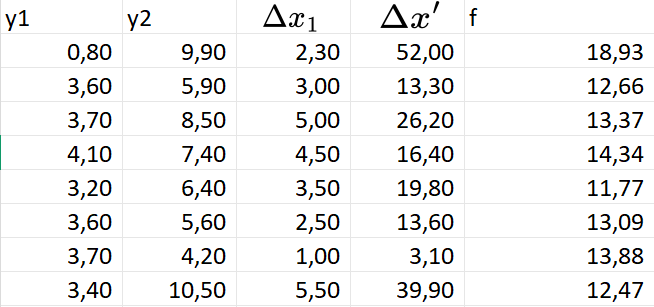
\includegraphics[scale=0.6]{таблица.png}
    \caption{таблица измерений(см)}
\end{figure}
Найдем среднее фокусное расстояние используя таблицу с n измерениями. Получим следующие результаты: $\langle f \rangle = 13,81$ см, $\sigma_{\langle f \rangle} = 0,51$.\\
\\
6. Для линзы 4.2 выпишем таблицу фокусных расстояний, измеренных различными методами.
\begin{table}[h!]
\centering
\begin{tabular}{|cl|c|c|}

\hline
\multicolumn{2}{|c|}{метод измерения}             & $\langle f \rangle$ & \textbackslash{}sigma\_\{$\langle f \rangle$\} \\ \hline
\multicolumn{2}{|c|}{подзорная труба}             & 12.5              & 0.09                                           \\ \hline
\multicolumn{2}{|c|}{Бессель}                     & 12.27               & 0.04                                           \\ \hline
\multicolumn{2}{|c|}{Бессель повернутый}          & 12.33               & 0.04                                           \\ \hline
\multicolumn{2}{|c|}{тонкая линза\_1}             & 11.92               & 0.05                                           \\ \hline
\multicolumn{2}{|c|}{тонкая линза\_2}             & 12.60               & 0.06                                           \\ \hline
\multicolumn{2}{|c|}{тонкая линза\_1\_повернутая} & 12.00               & 0.05                                           \\ \hline
\multicolumn{2}{|c|}{тонкая линза\_2\_повернутая} & 12.63               & 0.06                                           \\ \hline
\multicolumn{2}{|c|}{Аббе}                        & 13.81               & 0.51                                           \\ \hline
\end{tabular}
\end{table}
\section{Вывод}
В ходе данной работы были изучены методы определения фокусных расстояний линз и сложных оптических систем. Так, различными способами были как оценены, так и вычислены фокусные расстояния различных собирающихся линз(для линзы 4.2 были проделаны все методы). Все изученные методы давали значения фокусного расстояние, близкие друг к другу.
\end{document}